\documentclass{standalone}
\usepackage{tikz}
\usetikzlibrary{patterns, positioning}
\usepackage[sfdefault]{ClearSans} %% option 'sfdefault' activates Clear Sans as the default text font
\usepackage[T1]{fontenc}

\begin{document}
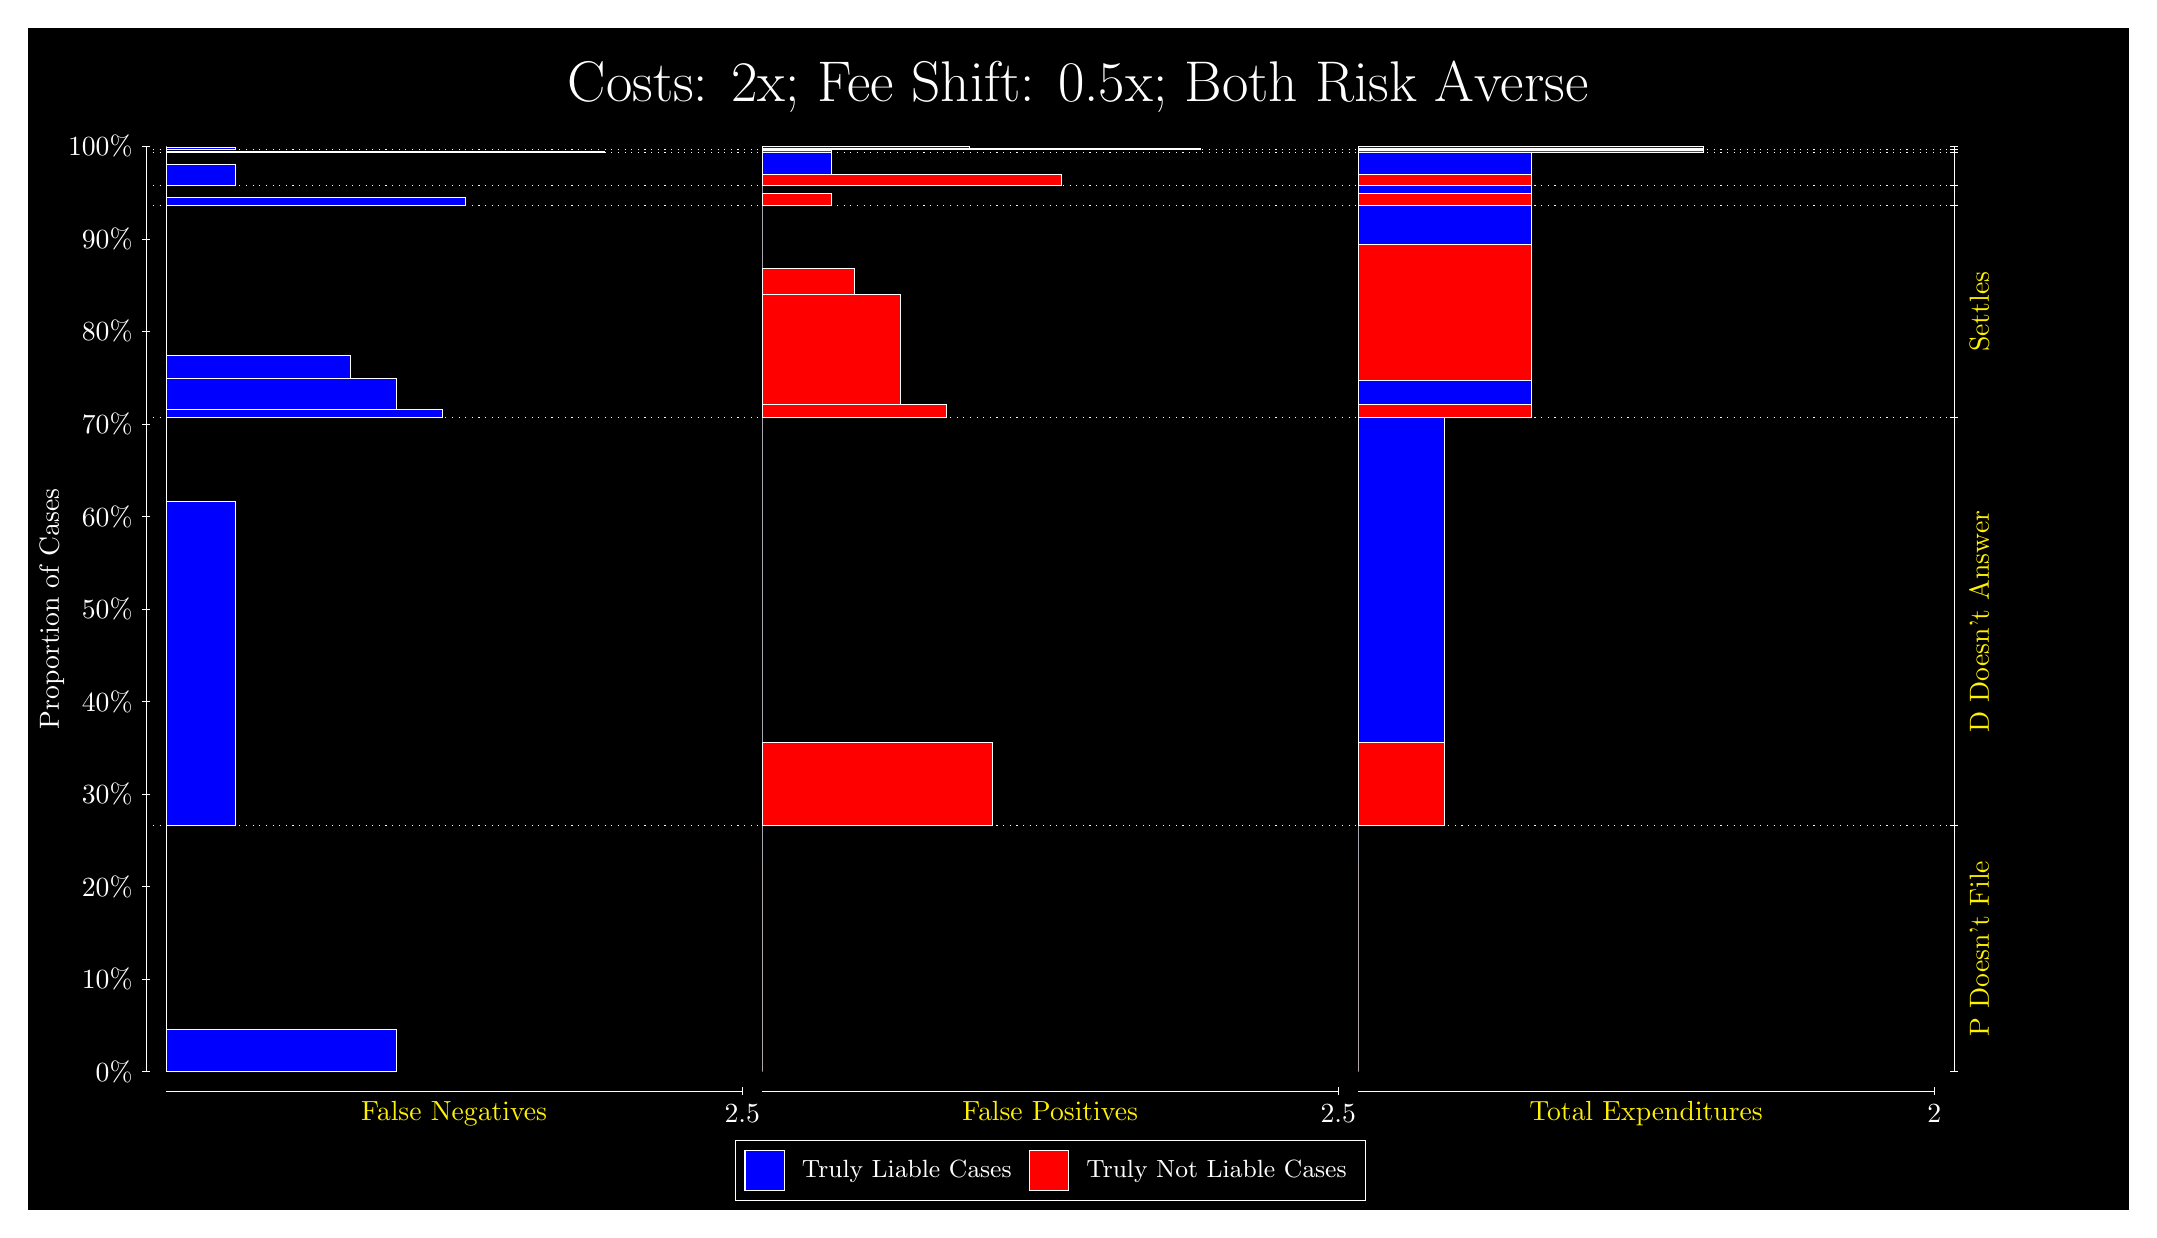
\begin{tikzpicture}
\draw[fill=black] (0,0) rectangle (26.667,15);
\draw[text=white] (0,13.5) rectangle (26.667,15) node[midway] {\huge Costs: 2x; Fee Shift: 0.5x; Both Risk Averse};
\draw[white, very thin] (1.5,1.75) -- (1.5,13.5);
\node[rotate=90, text=white, anchor=center] at (0.3, 7.625) {Proportion of Cases};
\draw[white, very thin] (1.45,1.75) -- (1.55,1.75);
\node[text=white, anchor=east] at (1.45, 1.75) {0\%};
\draw[white, very thin] (1.45,2.925) -- (1.55,2.925);
\node[text=white, anchor=east] at (1.45, 2.925) {10\%};
\draw[white, very thin] (1.45,4.1) -- (1.55,4.1);
\node[text=white, anchor=east] at (1.45, 4.1) {20\%};
\draw[white, very thin] (1.45,5.275) -- (1.55,5.275);
\node[text=white, anchor=east] at (1.45, 5.275) {30\%};
\draw[white, very thin] (1.45,6.45) -- (1.55,6.45);
\node[text=white, anchor=east] at (1.45, 6.45) {40\%};
\draw[white, very thin] (1.45,7.625) -- (1.55,7.625);
\node[text=white, anchor=east] at (1.45, 7.625) {50\%};
\draw[white, very thin] (1.45,8.8) -- (1.55,8.8);
\node[text=white, anchor=east] at (1.45, 8.8) {60\%};
\draw[white, very thin] (1.45,9.975) -- (1.55,9.975);
\node[text=white, anchor=east] at (1.45, 9.975) {70\%};
\draw[white, very thin] (1.45,11.15) -- (1.55,11.15);
\node[text=white, anchor=east] at (1.45, 11.15) {80\%};
\draw[white, very thin] (1.45,12.325) -- (1.55,12.325);
\node[text=white, anchor=east] at (1.45, 12.325) {90\%};
\draw[white, very thin] (1.45,13.5) -- (1.55,13.5);
\node[text=white, anchor=east] at (1.45, 13.5) {100\%};

\draw[white, very thin] (24.457,1.75) -- (24.457,13.5);
\draw[white, very thin] (24.407,1.75) -- (24.507,1.75);
\node[anchor=west] at (24.407, 1.75) {};
\draw[white, very thin] (24.407,4.8713) -- (24.507,4.8713);
\node[anchor=west] at (24.407, 4.8713) {};
\draw[white, very thin] (24.407,10.055) -- (24.507,10.055);
\node[anchor=west] at (24.407, 10.055) {};
\draw[white, very thin] (24.407,12.746) -- (24.507,12.746);
\node[anchor=west] at (24.407, 12.746) {};
\draw[white, very thin] (24.407,13.004) -- (24.507,13.004);
\node[anchor=west] at (24.407, 13.004) {};
\draw[white, very thin] (24.407,13.421) -- (24.507,13.421);
\node[anchor=west] at (24.407, 13.421) {};
\draw[white, very thin] (24.407,13.457) -- (24.507,13.457);
\node[anchor=west] at (24.407, 13.457) {};
\draw[white, very thin] (24.407,13.5) -- (24.507,13.5);
\node[anchor=west] at (24.407, 13.5) {};

\draw[white, very thin, fill=blue] (1.75,1.75) rectangle (4.6775,2.2872);
\draw[white, very thin, fill=red] (1.75,2.2872) rectangle (1.75,4.8713);
\draw[white, very thin, fill=blue] (1.75,4.8713) rectangle (2.6283,8.9979);
\draw[white, very thin, fill=red] (1.75,8.9979) rectangle (1.75,10.055);
\draw[white, very thin, fill=blue] (1.75,10.055) rectangle (5.2631,10.164);
\draw[white, very thin, fill=blue] (1.75,10.164) rectangle (4.6775,10.548);
\draw[white, very thin, fill=blue] (1.75,10.548) rectangle (4.092,10.849);
\draw[white, very thin, fill=red] (1.75,10.849) rectangle (1.75,12.746);
\draw[white, very thin, fill=blue] (1.75,12.746) rectangle (5.5558,12.847);
\draw[white, very thin, fill=red] (1.75,12.847) rectangle (1.75,13.004);
\draw[white, very thin, fill=blue] (1.75,13.004) rectangle (2.6283,13.277);
\draw[white, very thin, fill=red] (1.75,13.277) rectangle (1.75,13.421);
\draw[white, very thin, fill=blue] (1.75,13.421) rectangle (7.3123,13.434);
\draw[white, very thin, fill=red] (1.75,13.434) rectangle (1.75,13.457);
\draw[white, very thin, fill=blue] (1.75,13.457) rectangle (2.6283,13.487);
\draw[white, very thin, fill=red] (1.75,13.487) rectangle (1.75,13.5);
\draw[white, very thin, fill=red] (9.3189,1.75) rectangle (9.3189,4.334);
\draw[white, very thin, fill=blue] (9.3189,4.334) rectangle (9.3189,4.8713);
\draw[white, very thin, fill=red] (9.3189,4.8713) rectangle (12.246,5.9279);
\draw[white, very thin, fill=blue] (9.3189,5.9279) rectangle (9.3189,10.055);
\draw[white, very thin, fill=red] (9.3189,10.055) rectangle (11.661,10.223);
\draw[white, very thin, fill=red] (9.3189,10.223) rectangle (11.075,11.627);
\draw[white, very thin, fill=red] (9.3189,11.627) rectangle (10.49,11.952);
\draw[white, very thin, fill=blue] (9.3189,11.952) rectangle (9.3189,12.746);
\draw[white, very thin, fill=red] (9.3189,12.746) rectangle (10.197,12.903);
\draw[white, very thin, fill=blue] (9.3189,12.903) rectangle (9.3189,13.004);
\draw[white, very thin, fill=red] (9.3189,13.004) rectangle (13.125,13.148);
\draw[white, very thin, fill=blue] (9.3189,13.148) rectangle (10.197,13.421);
\draw[white, very thin, fill=red] (9.3189,13.421) rectangle (10.197,13.445);
\draw[white, very thin, fill=blue] (9.3189,13.445) rectangle (9.3189,13.457);
\draw[white, very thin, fill=red] (9.3189,13.457) rectangle (14.881,13.47);
\draw[white, very thin, fill=blue] (9.3189,13.47) rectangle (11.954,13.5);
\draw[white, very thin, fill=red] (16.888,1.75) rectangle (16.888,4.334);
\draw[white, very thin, fill=blue] (16.888,4.334) rectangle (16.888,4.8713);
\draw[white, very thin, fill=red] (16.888,4.8713) rectangle (17.986,5.9279);
\draw[white, very thin, fill=blue] (16.888,5.9279) rectangle (17.986,10.055);
\draw[white, very thin, fill=red] (16.888,10.055) rectangle (19.083,10.223);
\draw[white, very thin, fill=blue] (16.888,10.223) rectangle (19.083,10.524);
\draw[white, very thin, fill=red] (16.888,10.524) rectangle (19.083,12.253);
\draw[white, very thin, fill=blue] (16.888,12.253) rectangle (19.083,12.746);
\draw[white, very thin, fill=red] (16.888,12.746) rectangle (19.083,12.903);
\draw[white, very thin, fill=blue] (16.888,12.903) rectangle (19.083,13.004);
\draw[white, very thin, fill=red] (16.888,13.004) rectangle (19.083,13.148);
\draw[white, very thin, fill=blue] (16.888,13.148) rectangle (19.083,13.421);
\draw[white, very thin, fill=red] (16.888,13.421) rectangle (21.279,13.445);
\draw[white, very thin, fill=blue] (16.888,13.445) rectangle (21.279,13.457);
\draw[white, very thin, fill=red] (16.888,13.457) rectangle (21.279,13.47);
\draw[white, very thin, fill=blue] (16.888,13.47) rectangle (21.279,13.5);
\draw[white, dotted] (1.5,4.8713) -- (24.457,4.8713);
\draw[white, dotted] (1.5,10.055) -- (24.457,10.055);
\draw[white, dotted] (1.5,12.746) -- (24.457,12.746);
\draw[white, dotted] (1.5,13.004) -- (24.457,13.004);
\draw[white, dotted] (1.5,13.421) -- (24.457,13.421);
\draw[white, dotted] (1.5,13.457) -- (24.457,13.457);
\draw[white, very thin] (1.75,1.5) -- (9.0689,1.5);
\node[text=yellow, anchor=north] at (5.4094, 1.5) {False Negatives};
\draw[white, very thin] (9.0689,1.45) -- (9.0689,1.55);
\node[text=white, anchor=north] at (9.0689, 1.45) {2.5};

\draw[white, very thin] (9.3189,1.5) -- (16.638,1.5);
\node[text=yellow, anchor=north] at (12.978, 1.5) {False Positives};
\draw[white, very thin] (16.638,1.45) -- (16.638,1.55);
\node[text=white, anchor=north] at (16.638, 1.45) {2.5};

\draw[white, very thin] (16.888,1.5) -- (24.207,1.5);
\node[text=yellow, anchor=north] at (20.547, 1.5) {Total Expenditures};
\draw[white, very thin] (24.207,1.45) -- (24.207,1.55);
\node[text=white, anchor=north] at (24.207, 1.45) {2};

\node[text=yellow, centered, rotate=90] at (24.777, 3.3106) {P Doesn't File};
\node[text=yellow, centered, rotate=90] at (24.777, 7.4629) {D Doesn't Answer};
\node[text=yellow, centered, rotate=90] at (24.777, 11.4) {Settles};





\draw (12.978300999999998,1.5) node[draw=none] (baseCoordinate) {};
\begin{scope}[align=center]
        \matrix[scale=0.5, draw=white, below=0.5cm of baseCoordinate, nodes={draw}, column sep=0.1cm]{
            \node[rectangle, draw, minimum width=0.5cm, minimum height=0.5cm, fill=blue] {}; &
            \node[draw=none, font=\small, text=white] (B) {Truly Liable Cases}; &
            \node[rectangle, draw, minimum width=0.5cm, minimum height=0.5cm, fill=red] {}; &
            \node[draw=none, font=\small, text=white] (B) {Truly Not Liable Cases}; \\
            };
\end{scope}

\end{tikzpicture}
\end{document}